\section{密钥封装机制(KEM)概述}

KEM 是一种基于公钥密码学的密钥交换机制,使得通信双方可以在一定条件下构建共享秘密密钥,可以使用在接下来的对称加密环节。

一个 KEM 主要由三部分组成,分别是
\begin{itemize}
  \item KeyGen:概率性算法,生成公私钥对。
  \item Encaps:概率性算法,生成密文和共享密钥。
  \item Decaps:确定性算法,根据密文和私钥生成共享密钥。
\end{itemize}

\begin{figure}[ht]
  \centering
  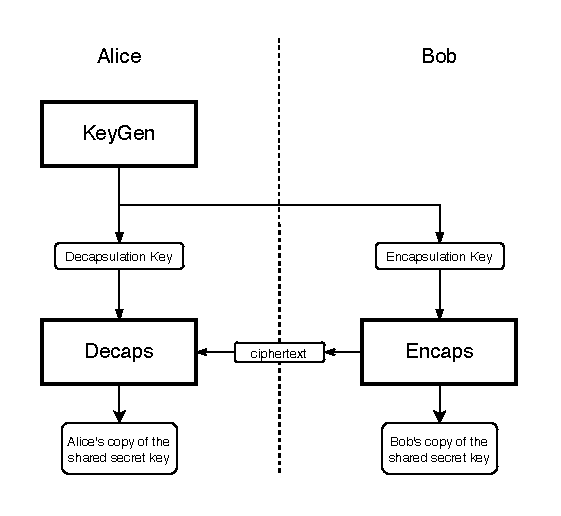
\includegraphics[width=0.5\textwidth]{doc/graph/KEM.drawio.pdf}
  \caption{KEM 工作流程图}
\end{figure}

由于 KEM 在 Decaps 阶段生成的共享密钥是确定性的,因此 KEM 通常会在 Encaps 阶段引入随机性,以避免密文的重放攻击。不同的 KEM 实现可能导致 Decaps 无法生成共享密钥,导致密文无法解密,通常会选择合适的参数,以保证发生这种情况的概率足够小。